\section{Giới thiệu}
Các mạng học sâu (DNNs) là mô hình học máy cực kỳ mạnh mẽ đạt được hiệu suất tuyệt vời đối với các vấn đề khó khăn như nhận dạng giọng nói \citep{hinton2012deep, DBLP:journals/taslp/DahlYDA12} và nhận dạng đối tượng trực quan \citep{DBLP:journals/cacm/KrizhevskySH17, DBLP:conf/cvpr/CiresanMS12, lecun1998gradient, LeRMDCCDN12}. DNNs rất mạnh mẽ vì chúng có thể thực hiện tính toán song song tùy ý với một vài bước tối thiểu nhất. Một ví dụ đáng ngạc nhiên về sức mạnh của DNNs là khả năng sắp xếp N số bit N của chúng chỉ bằng cách sử dụng 2 lớp ẩn có kích thước bậc hai \citep{DBLP:conf/swat/Razborov92}. Vì vậy, trong khi mạng nơ-ron có liên quan đến các mô hình thống kê thông thường, chúng lại học phép tính một cách phức tạp. Hơn nữa, các mạng DNNs lớn được huấn luyện lan truyền ngược có giám sát bất cứ khi nào tập huấn luyện được gắn nhãn có đủ thông tin để chỉ định các tham số của mạng. Do đó, nếu tồn tại một tham số hiệu chỉnh của một mạng DNNs lớn mà mạng đó đạt được kết quả tốt (ví dụ: vì con người có thể giải quyết công việc rất nhanh), thì lan truyền ngược có giám sát sẽ tìm ra các tham số này và giải quyết vấn đề.

Mặc dù DNNs có tính linh hoạt, nhưng DNNs chỉ có thể được áp dụng cho các vấn đề mà đầu vào và mục tiêu đầu ra có thể được mã hóa hợp lý bằng các vectơ có chiều cố định. Đó là một hạn chế đáng kể, vì nhiều vấn đề quan trọng được thể hiện tốt nhất với các trình tự mà độ dài của nó không được biết trước. Ví dụ, nhận dạng giọng nói và dịch máy là các vấn đề tuần tự. Tương tự như vậy, trả lời câu hỏi cũng có thể được coi là ánh xạ một chuỗi các từ đại diện cho câu hỏi với một chuỗi các từ đại diện cho câu trả lời. Do đó, rõ ràng rằng một phương pháp độc lập với miền học cách ánh xạ các chuỗi thành các chuỗi sẽ hữu ích.

Các chuỗi tuần tự đặt ra một thách thức đối với các DNNs vì chúng yêu cầu rằng kích thước của các đầu vào và đầu ra phải được biết và cố định. Bài nghiên cứu này chỉ ra một ứng dụng đơn giản của kiến trúc Bộ nhớ Gần-Xa (LSTM) \citep{HochreiterandSchmidhuber1997} có thể giải quyết các vấn đề tuần tự tổng quát. Ý tưởng là sử dụng một LSTM để đọc chuỗi đầu vào, một bước thời gian tại một thời điểm, để biểu diễn vectơ có chiều cố định lớn và sau đó sử dụng một LSTM khác để trích xuất chuỗi đầu ra từ vectơ đó. LSTM thứ hai về cơ bản là một mô hình ngôn ngữ mạng nơ-ron hồi quy \citep{Mikolov2010} ngoại trừ việc nó được điều chỉnh dựa trên chuỗi tuần tự đầu vào. Khả năng học thành công trên dữ liệu có phạm vi dài phụ thuộc vào thời gian của LSTM khiến nó trở thành lựa chọn đương nhiên cho ứng dụng này do độ trễ thời gian đáng kể giữa đầu vào và đầu ra tương ứng của chúng.

\begin{figure}
	\centering
	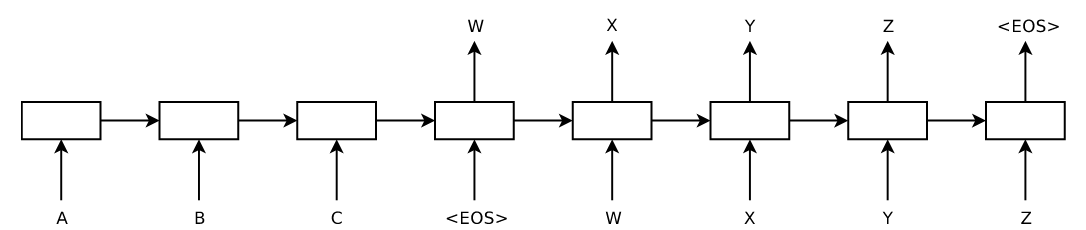
\includegraphics[scale=0.3]{img/fig1.png}
	\caption{Mô hình đọc chuỗi đầu vào ABC và tạo chuỗi đầu ra WXYZ.}
	\label{fig_1}
\end{figure}
